\chapter{Sprint 5 : Optimisation du temps d'exécution de la pipeline de Projet "Scribe"}
\section{Introduction}
Après avoir établi les bases d'une chaîne (CI/CD) au cours du quatriéme sprint, ce sprint se concentrera sur l'optimisation du temps d'exécution de la pipeline de déploiement pour le projet "Scribe". Cette étape est cruciale pour améliorer d'avantage l'efficacité du processus de déploiement. Dans ce chapitre, nous explorons les objectifs, le backlog, les étapes de réalisation et les résultats obtenus au cours de ce sprint.\\

\section{Analyse des besoins}
Dans cette section, nous allons aborder les objectifs et le backlog de ce sprint.
\subsection{Objectif de sprint 5}
L'objectif fondamental de ce sprint est d'optimiser le temps d'exécution de la pipeline de déploiement du projet "Scribe". Actuellement, la durée de la chaîne CI/CD peut représenter un frein significatif, ralentissant la mise à disposition de nouvelles fonctionnalités. En optimisant la vitesse de passage de chaque étape de la pipeline, nous visons à fournir des avantages tangibles en termes de réactivité, de livraison rapide et de satisfaction globale de l'équipe de développement.

\subsection{Backlog Sprint 5}
\normalsize{Afin de bien organiser le travail durant ce sprint, nous allons établir le Backlog du sprint 5 illustré par le tableau \ref{tab:sprintBacklog5}.
\newpage
\begin{longtable}{|>
{\centering}m{0.085\linewidth}|>
{\centering}m{0.3\linewidth}|>{\centering}m{0.085\linewidth}|>
{\centering}m{0.2\linewidth}|c|}
\hline
ID User Story & User story & ID tâche & Tâche & Priorité \\
\hline
\multirow{3}{*}{5.1} & \multirow{3}{\linewidth}{ {En tant que développeur, je veux pouvoir livrer des mises à jour
des nouvelles fonctionnalités plus rapide.}} & 5.1.1 &  Faire les modification nécessaire au niveau gitlab ci. & Haute \\ 
\cline{3-5}
      & & 5.1.2 & Tester l'impact des modifications sur la durée d'exécution. & Moyenne \\
\hline
\caption{Backlog du Sprint 4}
\label{tab:sprintBacklog5}
\end{longtable}
\section{Analyse du Branch Master}
Au sein du processus de déploiement du projet Scribe, un problème majeur a été identifié lors de l'exécution du job "Preinstall" via Ansible. Ce probléme réside dans la gestion des group\_vars (variables de groupe) et des environnements (ENV) lors de l'exécution du playbook.\\
Pour illustrer ce problème,la figure \ref{figlog} montre clairement l'exécution du job "Preinstall" avec les group\_vars "as" et l'environnement "QPM" définis comme prévus. Cependant, ce qui est préoccupant, c'est que le job semble également traiter d'autres group\_vars et environnements qui ne sont pas requis pour cette tâche spécifique.
\begin{figure}[htbp]
     \centering
  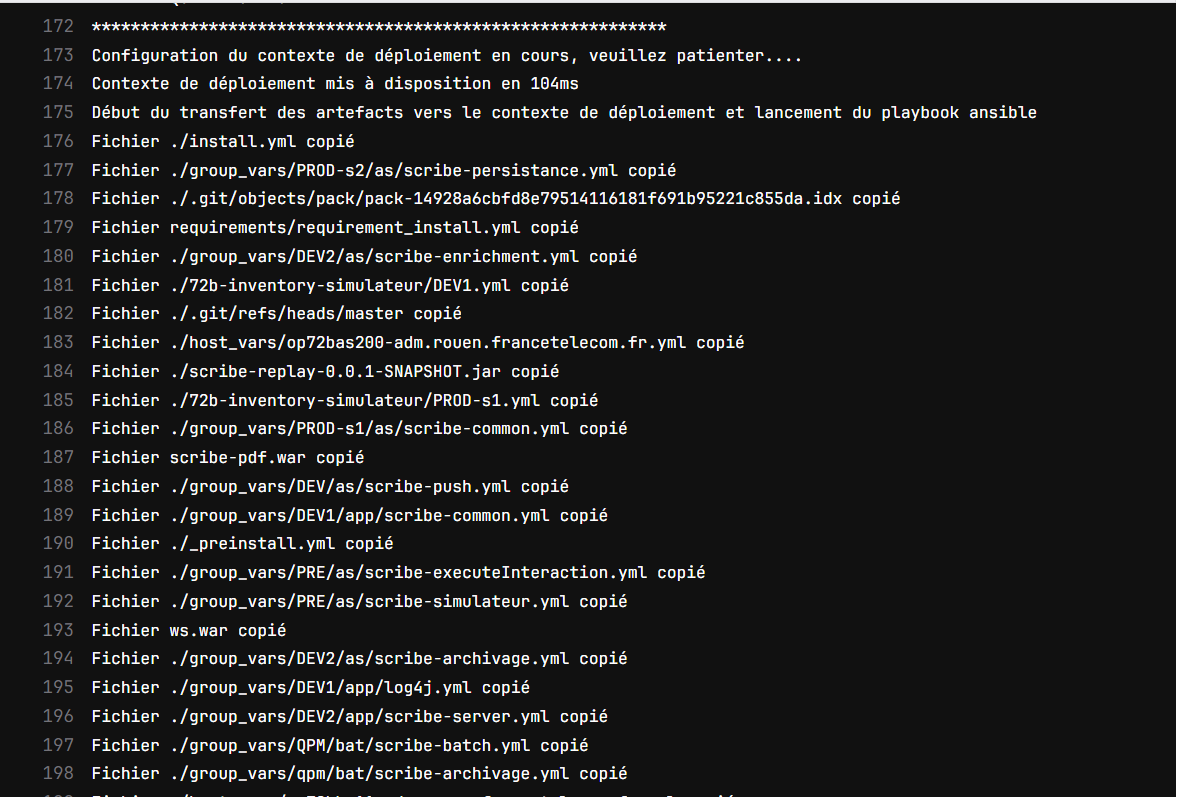
\includegraphics[scale=0.5]{img/faraaaaah2.png}
        \caption{Log du job "Preinstall" avec les group\_vars "as" et l'environnement "QPM"} 
  \label{figlog}
 \end{figure}
 \newpage
 Dans la figure \ref{figlog} , on peut observer que les group\_vars "app" et "bat" sont également traités bien que cela ne soit pas nécessaire pour le job "Preinstall" en cours. De plus, les environnements "PRE", "dev1" et "dev2" sont également pris en compte, bien que seul "QPM" soit pertinent pour cette opération.\\
 Cette situation soulève plusieurs problèmes.le traitement des group\_vars et des environnements inutiles ajoute une surcharge de travail non nécessaire au processus de déploiement. Cela signifie que des ressources précieuses sont utilisées pour traiter des données qui ne contribuent pas à la tâche en cours, ce qui retarde l'ensemble du processus.\\

la figure \ref{figtemps} montre le Temps d'exécution du job "preinstall" pour le groupe "As" et l'environnement "QPM" qui a duré 2 minutes 38 secondes.
\begin{figure}[htbp]
     \centering
  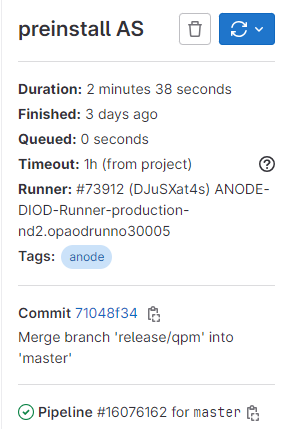
\includegraphics[scale=0.7]{img/master scribe.png}
        \caption{le temps d'execution du job "Preinstall AS"} 
  \label{figtemps}
 \end{figure}
\section{Réalisation}
Pour résoudre ce problème, nous avons apporté des modifications significatives à la configuration de la pipeline. Désormais, lorsqu'on lance la pipeline avec le groupe\_vars "As" et l'environnement "DEV", seuls ces paramètres spécifiques sont chargés, comme en témoigne une capture ultérieure du temps d'exécution du job "preinstall".\\

Un élément clé de notre solution était de rendre dynamiques et variables les liens vers les fichiers d'environnement et de groupe situés sous le répertoire "ansible". Au lieu d'utiliser des chemins statiques, nous avons introduit des variables telles que "environnement" et "group" pour définir dynamiquement les chemins vers les fichiers appropriés en fonction du déploiement en cours. Cette variabilisation nous a permis de charger uniquement les éléments pertinents, réduisant ainsi le temps de chargement global.

Nous avons observé dans la figure \ref{figlogop} lors de l'exécution du job "preinstall" avec les paramètres du groupe\_vars "As" et de l'environnement "DEV". Les résultats de cette exécution étaient remarquables. Conformément à notre objectif d'optimisation, seuls les paramètres spécifiques du groupe\_vars "As" et de l'environnement "DEV" ont été chargés

\begin{figure}[htbp]
     \centering
  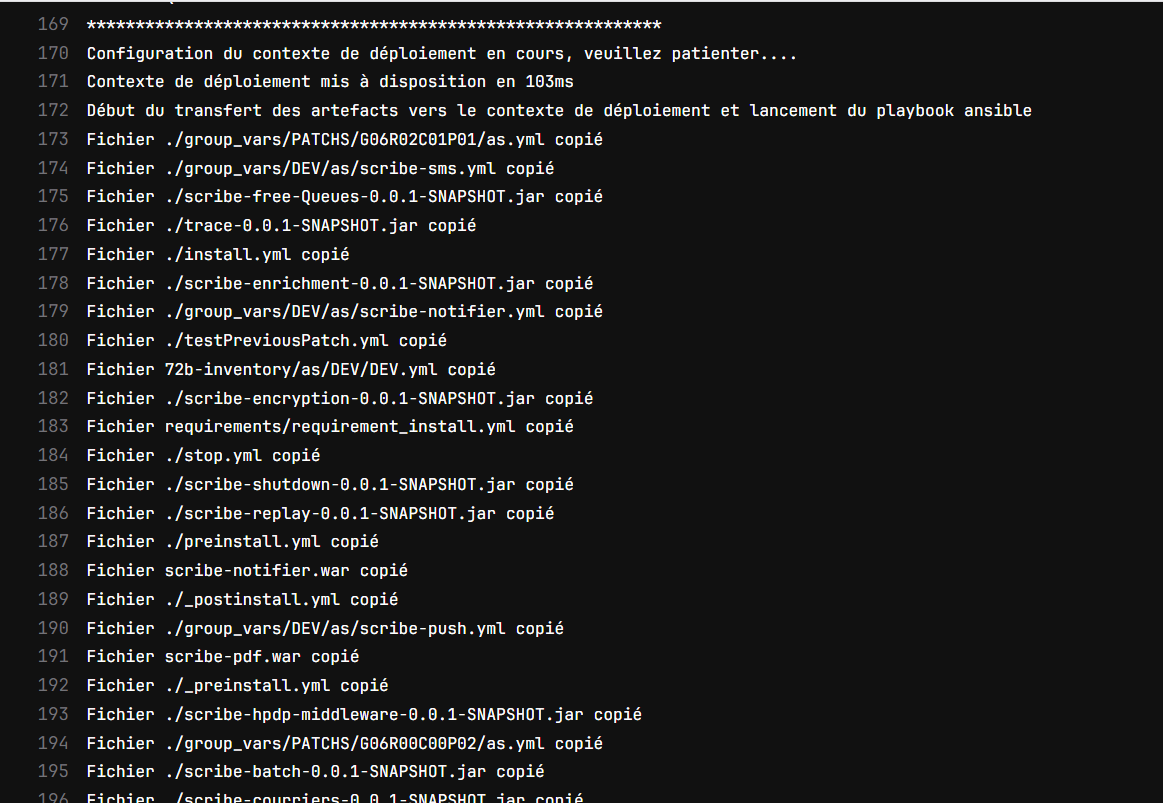
\includegraphics[scale=0.5]{img/faraaah1.png}
        \caption{Log du job "Preinstall" avec les group\_vars "as" et l'environnement "QPM"} 
  \label{figlogop}
 \end{figure}
 la figure \ref{tempsss} montre le Temps d'exécution du job "preinstall" pour le groupe "As" et l'environnement "QPM" qui a duré 1 minutes 24 secondes.\\
 \begin{figure}[htbp]
     \centering
  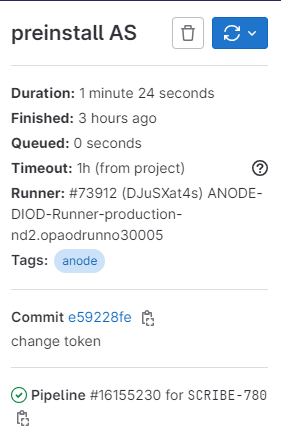
\includegraphics[scale=0.56]{img/Capture.PNGop scribe 780.png}
        \caption{le temps d'execution du job "Preinstall AS"} 
  \label{tempsss}
 \end{figure}
 \newpage
Les réalisations obtenues dans le cadre de cette optimisation de la 
pipeline sont incontestablement positives. Notre capacité à charger 
uniquement les group\_vars "As" et l'environnement "DEV" lors de 
l'exécution de la pipeline, tout en éliminant les traitements 
superflus, a abouti à une réduction significative du temps 
d'exécution du job "preinstall". Le passage de 2 minutes 38 secondes 
à seulement 1 minute 24 secondes démontre l'efficacité de notre 
démarche.
\\
Cette optimisation contribuera non seulement à accélérer les cycles 
de déploiement, mais elle renforcera également la cohérence et la 
fiabilité de nos installations. Elle témoigne de notre engagement à 
mettre en place des processus plus efficaces et à maximiser 
l'utilisation de nos ressources. Ces améliorations auront un impact 
positif sur l'ensemble de notre processus de développement, nous 
permettant de fournir des résultats plus rapides et plus fiables à 
nos utilisateurs et à notre équipe.

\section{Conclusion}
La réalisation de ce sprint a abouti à une optimisation réussie du temps d'exécution de la pipeline de déploiement du projet Scribe. En variabilisant les liens vers les environnements et les groupes, nous avons réussi à réduire considérablement les délais de chargement et à améliorer l'efficacité du déploiement. Cette réalisation témoigne de notre engagement à maximiser l'efficacité de nos processus de développement et de déploiement, tout en contribuant à l'amélioration globale de la productivité de l'équipe.
